\section{Aufbau des Systems}
\subsection{Hardwareaufbau}
Ein Steuerrad, drei Pedalen, ein Schaltknüppel und diverse Knöpfen dienen als Eingabegeräte für den Fahrsimulator. Diese sind über USB mit einem Computer verbunden. Als Ausgabe dient ein leistungsstarker Projektor, der das Bild auf eine hochreflektierende Projektionsfläche projiziert.

\begin{figure}[H]
\centering 
\includegraphics[width=0.6\linewidth]{src/foto_hardware_aufbau.png}
\caption{Hardwareaufbau mit Steuerrad und Pedalen} % Titel der Grafik
\label{Hardwareaufbau} % Labelname
\end{figure}

\newpage

\subsection{Systembeschreibung}

% Bild für Systembeschreibung
\begin{figure}[H]
\centering 
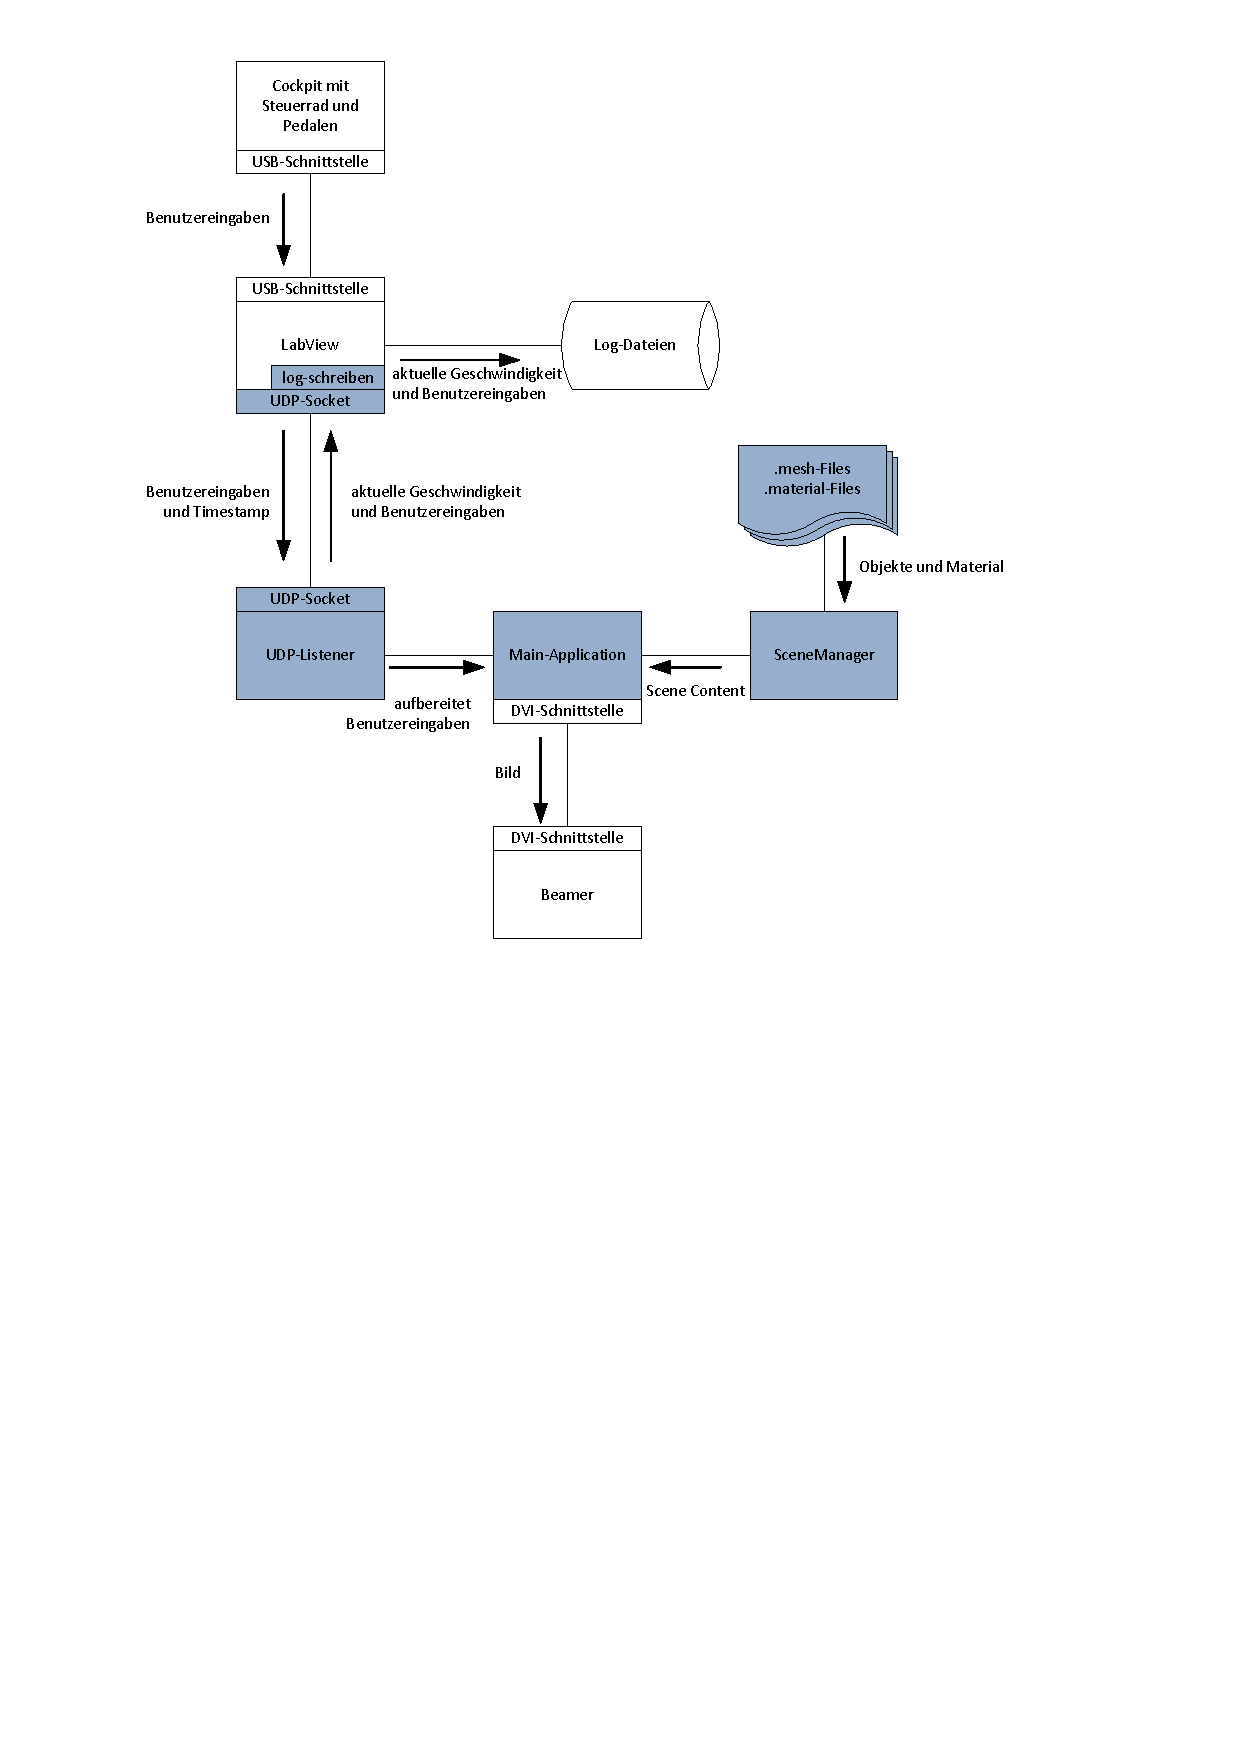
\includegraphics[width=1\linewidth]{src/Systembeschreibung.pdf}
\caption{Systembeschreibung} % Titel der Grafik
\label{Systembeschreibung} % Labelname
\end{figure}

Die blau markierten Komponenten in Abbildung \ref{Systembeschreibung} werden im Rahmen dieser Projektarbeit entwickelt. Alle übrigen sind bereits vorbestehend. \\
Benutzereingaben, die im Cockpit gemacht werden, werden von einem \gls{labview}-Programm eingelesen. Dieses benötigt einen UDP-Socket, über den verschiedene Eingaben an die Simulationssoftware weitergeleitet werden. Es handelt sich hierbei um Werte, die das Drehen des Steuerrads und den Druck auf Gas- oder Bremspedal quantifizieren. Zusätzlich wird ein zweiter UDP-Socket für das Empfangen diverser Informationen, die von unserem Programm gesendet werden, verwendet. Die empfangenen Daten werden vom \gls{labview}-Programm in ein Log-File geschrieben.\\
Weiter muss in C++ ein UDP-Socket mit entsprechendem UDP-Listener implementieren werden, um die Benutzereingaben zu empfangen. Der UDP-Listener wird gleichzeitig dazu verwendet, die Geschwindigkeit des Fahrzeugs sowie Timestamps und weitere Daten an das \gls{labview}-Programm zurück zu schicken. Damit können die Daten gespeichert und später ausgewertet werden.\\
Diese Aufteilung durch eine Netzwerkschnittstelle ermöglicht es,  das System, wenn notwendig, zu dezentralisieren. Einfachheitshalber wird der UDP-Listener erst in einem Video-Beispiel implementiert und getestet (Siehe Anhang \ref{sec:videoplayer}). Nachfolgend wird er in das Programm des Fahrsimulators integriert.\\
Sind die Daten vom UDP-Listener empfangen und aufbereitet, werden sie im Hauptprogramm weiter verwendet. Während die Position des Steuerrades, des Gas- und Bremspedales vom UDP-Listener permanent an das Hauptprogramm übertragen werden, wertet dieses die Positionen aus und veranlasst die entspechenden Aktionen in der geladenen Szene. 
Die Szene selbst wird von einem Szenen-Manager geladen. Die berechnete Szene wird schlussendlich in einem Fenster des Hauptprogramms angezeigt und über eine DVI-Schnittstelle an den Projektor übertragen.

\subsection{Anforderungen}
\subsubsection{Funktionale Anforderungen}
\begin{itemize}
\item Der Fahrsimulator ermöglicht es dem Probanden, vom Cockpit aus das Fahrzeug zu steuern. Der Proband blickt durch die Frontscheibe des Fahrzeugs und fährt auf der Strasse.
\item Die aktuelle Geschwindigkeit des gesteuerten Fahzeuges soll für den Probanden ersichtlich sein. 
\item Es sollen dem Fahrsimulator zwei Szenen zur Verfügung stehen. Die eine Szene stellt eine Stadt dar, die andere eine Berglandschaft mit Tunnels.
\item Die Manipulationen des Benutzers und wichtige Parameter, wie z.B. Geschwindigkeit, werden in einer Datei fortlaufend abgespeichert.
\item Alle ein- und ausgehenden Parameter des Systems werden in \gls{labview} grafisch dargestellt.
\end{itemize}

\subsubsection {Nicht funktionale Anforderungen}
\renewcommand{\labelenumi}{\alph{enumi})}

\begin{itemize}
\item Das System ist robust. Es muss auch bei Fehleingaben weiter laufen. 
\item Das Starten des Fahrsimulator wird einfach gehalten.
\item Das Fahrzeughandling ist realitätsnah.
\item Der Fahrsimulator bietet dem Probanden eine realistische Fahrsimulation inklusive Strassen, Gebäude und Verkehrsschilder. 
\item Die Reaktionszeit des Systems ist möglichst kurz. Die Verzögerungen sind mess- und kalkulierbar.
\item Das System ist modular aufgebaut, um später einfach erweitert werden zu können.
\item Das System funktioniert auf der existierender Hardware, und läuft auch wenn Teile des Fahrsimulators ausgetauscht werden.
\end{itemize}
